\section{MPI Communication}
The Message Passing Interface (MPI)  is a commonly employed standard in high-performance computing (HPC) for programming distributed memory systems. 
Instead of offering an implementation, MPI serves as an application programming interface (API), comprising functions, constants, and expected behaviors. 
Various vendors offer their own implementations of this API, such as Open MPI.\\
MPI operations consist of a sequential sequence of steps: initialization, starting, completion, and freeing. 
These actions can be carried out in one or more MPI procedures and are carried out by the MPI library. The many forms of communication are thoroughly explained in the paragraphs that follow.\\

\subsection{Point-to-point Communications and Collective Communication.}
In general, MPI offers three different communication paradigms determining how processes communicate with the others: point-to-point, one-sided, and collective communication.
Point-to-point (P2P) communication is the simplest form, as it only involves exactly two processes, which both actively take part in the communication. 
One process sends a message (e.g., using \texttt{MPI\_Send}), which the receive process receives with a corresponding receive call (e.g., \texttt{MPI\_Recv}).
One-sided communication also involves two processes, but only one of them has to actively take part in the communication. This work does not focus on one-sided communication, so it will not be discussed in detail.\\
Finally, collective communication entails the exchange of messages among multiple processes. 
For instance, an individual process can broadcast a message to all other processes within the same group, utilizing the \texttt{MPI\_Bcast} function. 
Every collective communication can be implemented through peer-to-peer communication calls.

\subsection{Blocking and non-blocking communication.}
In blocking communication, four steps (initialization, starting, completion and freeing) are combined into single one and must be performed sequentially without interrupt. 
A state transition diagram for blocking operations is shown in \autoref{fig:mpi_blocking}.
\begin{figure}[h!]
    \centering
    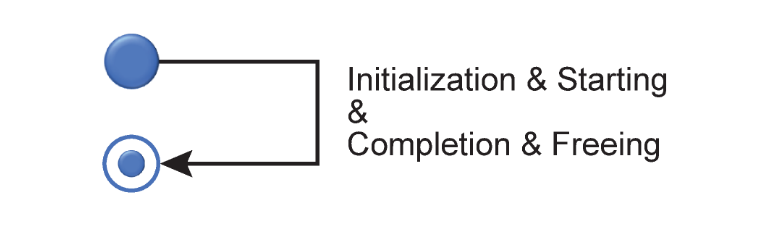
\includegraphics[width=0.5\textwidth]{pictures/mpi_blocking.png}
    \caption{State transition diagram for blocking operations. \cite{noauthor_mpi_nodate}}
    \label{fig:mpi_blocking}    
\end{figure}

Blocking means that the MPI primitive waits until the message buffer containing the data being sent/received is safe to be used again by the calling process. 
Only then is control returned to the caller.
On send, actual implementations of \texttt{MPI\_Send} may either block until all data has been transmitted or copy the data to an intermediate internal buffer. 
The use of blocking primitives may be prone to deadlocks, if programmers do not carefully consider send and receive order.
\texttt{MPI\_Isend} and \texttt{MPI\_Irecv} are non-blocking message communication. 
Compared to \texttt{MPI\_Send}'s arguments, \texttt{MPI\_Isend} adds an additional argument for a request handle. The handle is used in calls to \texttt{MPI\_Wait} to identify which send to wait for.\\
The non-blocking process combines the initialization and starting phases into a single procedure call that does not block, while the completion and freeing stages are handled in a separate procedure call, which can be either blocking or non-blocking.
A state transition diagram for non-blocking operations is shown in \autoref{fig:mpi_non_blocking}.\\
\begin{figure}[h!]
    \centering
    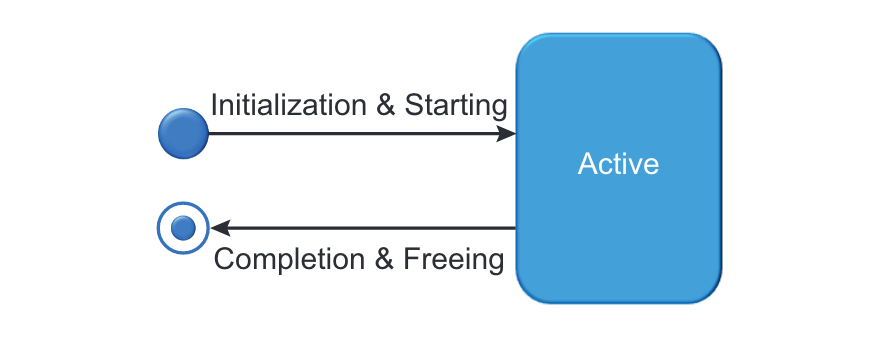
\includegraphics[width=0.5\textwidth]{pictures/mpi_non-blocking.png}
    \caption{State transition diagram for non-blocking operations. \cite{noauthor_mpi_nodate}}
    \label{fig:mpi_non_blocking}
\end{figure}
Non-blocking calls return immediately after initiating the communication and the user thread can execute more operations, eventually followed by a completion operation (a wait or test) on the request. The communication is considered complete after a successful call to \texttt{MPI\_Wait} (or \texttt{MPI\_Test}, etc.). 
Non-blocking is used to help promote overlap communication and computation, resulting in communicating cost hiding and yielding overall better performance on systems that support it. To avoid tampering with the data, programmers must ensure that the message data is not modified before the communication is completed.
